\subsection{监控介绍}

在腾讯开悟平台的训练管理页面,提供了查看监控功能,点击后,即可在新标签页中打开监控面板,如下图所示。可以通过查看监控数据实时定位自己的训练进程,从而帮助大家评更快更准确的找到问题所在。

\subsubsection{监控面板介绍}

在监控面板中,包括 错误日志数量 和 监控指标图 两部分内容。

错误日志数量:在该模块中,可以看到训练过程中每个模块的错误日志数量。点击模块卡片可以进入日志详情页,查看该模块的错误日志信息。

监控指标图:在该模块中,可以看到四类数据指标,分别是basic(基础指标)、algorithm(算法指标)、env(环境指标)、diy(自定义指标)。

\begin{table}[H]
    \begin{tabularx}{1\textwidth}{ l X } % | 表示垂直边框
        \hline % 水平边框
        \textbf{指标分类} & \textbf{说明}  \\
        \hline
        basic&包括强化学习训练过程中的标准数据和资源使用数据。\\
        algorithm&和算法相关的数据指标,不同算法上报的指标可能会有所不同。\\
        env&和环境相关的数据指标,不同环境上报的指标不同。\\
        diy&用户自行上报的数据指标。\\
        \hline
    \end{tabularx}

    \centering
    \caption{监控面板}
    \label{monitor-dashboard}
\end{table}


\begin{enumerate}
    \item 基础指标

\begin{table}[H]
    \begin{tabularx}{1\textwidth}{ l X } % | 表示垂直边框
        \hline % 水平边框
        \textbf{指标名称} & \textbf{说明}  \\
        \hline
    train\_global\_step&训练的累计步数,即agent.learn的调用次数。取决于各算法的具体实现:DQN系列的算法从样本池中采样一次后调用agent.learn。\\
    predict\_succ\_cnt&采样预测的累计帧数,即agent.predict的调用次数。\\
    sample\_production\_and\_consumption\_ratio&等于训练步数除以采样预测的累计帧数。\\
    episode\_cnt&已经结束的任务个数。\\
    load\_model\_succ\_cnt&预测加载模型文件成功的次数,即调用agent.load\_model的调用次数。\\
    sample\_receive\_cnt&learner成功接收的样本数量。\\
        \hline
    \end{tabularx}
    \centering
    \caption{基础指标}
    \label{monitor-basic}
\end{table}


    \item 算法指标

\begin{table}[H]
    \begin{tabularx}{1\textwidth}{ l X } % | 表示垂直边框
        \hline % 水平边框
        \textbf{指标名称} & \textbf{说明}  \\
        \hline
        reward&累积回报,反应了智能体的能力,正常训练情况下指标应该是震荡向上。\\
        q\_value&target网络的Q值,一定程度反应Q值的稳定性。\\
        value\_loss&计算loss的标量值,反应训练的进程,正常情况下指标应该是逐渐接近于0。\\
        \hline
    \end{tabularx}
    \centering
    \caption{算法指标}
    \label{monitor-alg}
\end{table}

    \item 环境指标

\begin{table}[H]
    \begin{tabularx}{1\textwidth}{ l X } % | 表示垂直边框
        \hline % 水平边框
        \textbf{指标名称} & \textbf{说明}  \\
        \hline
        score & 该面板包含两个指标:total\_score:任务结束时的得分,若任务超时,则该局得分为0。treasure\_score:任务结束时收集到的宝箱奖励。\\
        steps & 该面板包含两个指标:max\_steps:任务设置的最大步数。finished\_steps:任务结束时所用的步数。若任务超时,则该局完成步数等于最大步数。\\
        treasure & 该面板包含两个指标:total\_treasures:任务设置的宝箱个数。collected\_treasures:任务结束时收集到的宝箱个数。\\
        treasure\_random & 宝箱是否随机。若为0则表示宝箱位置固定,若为1则表示宝箱位置随机。\\
        skill\_cnt & 技能使用次数。\\
        buff\_cnt & 加速增益拾取次数。\\
        \hline
    \end{tabularx}
    \centering
    \caption{环境指标}
    \label{monitor-env}
\end{table}

    \item diy(自定义指标)

    我们提供了五个自定义指标diy\_1至diy\_5以便用户可以上报自己想要监控的数据。

    \begin{figure}[H]
        \centering
        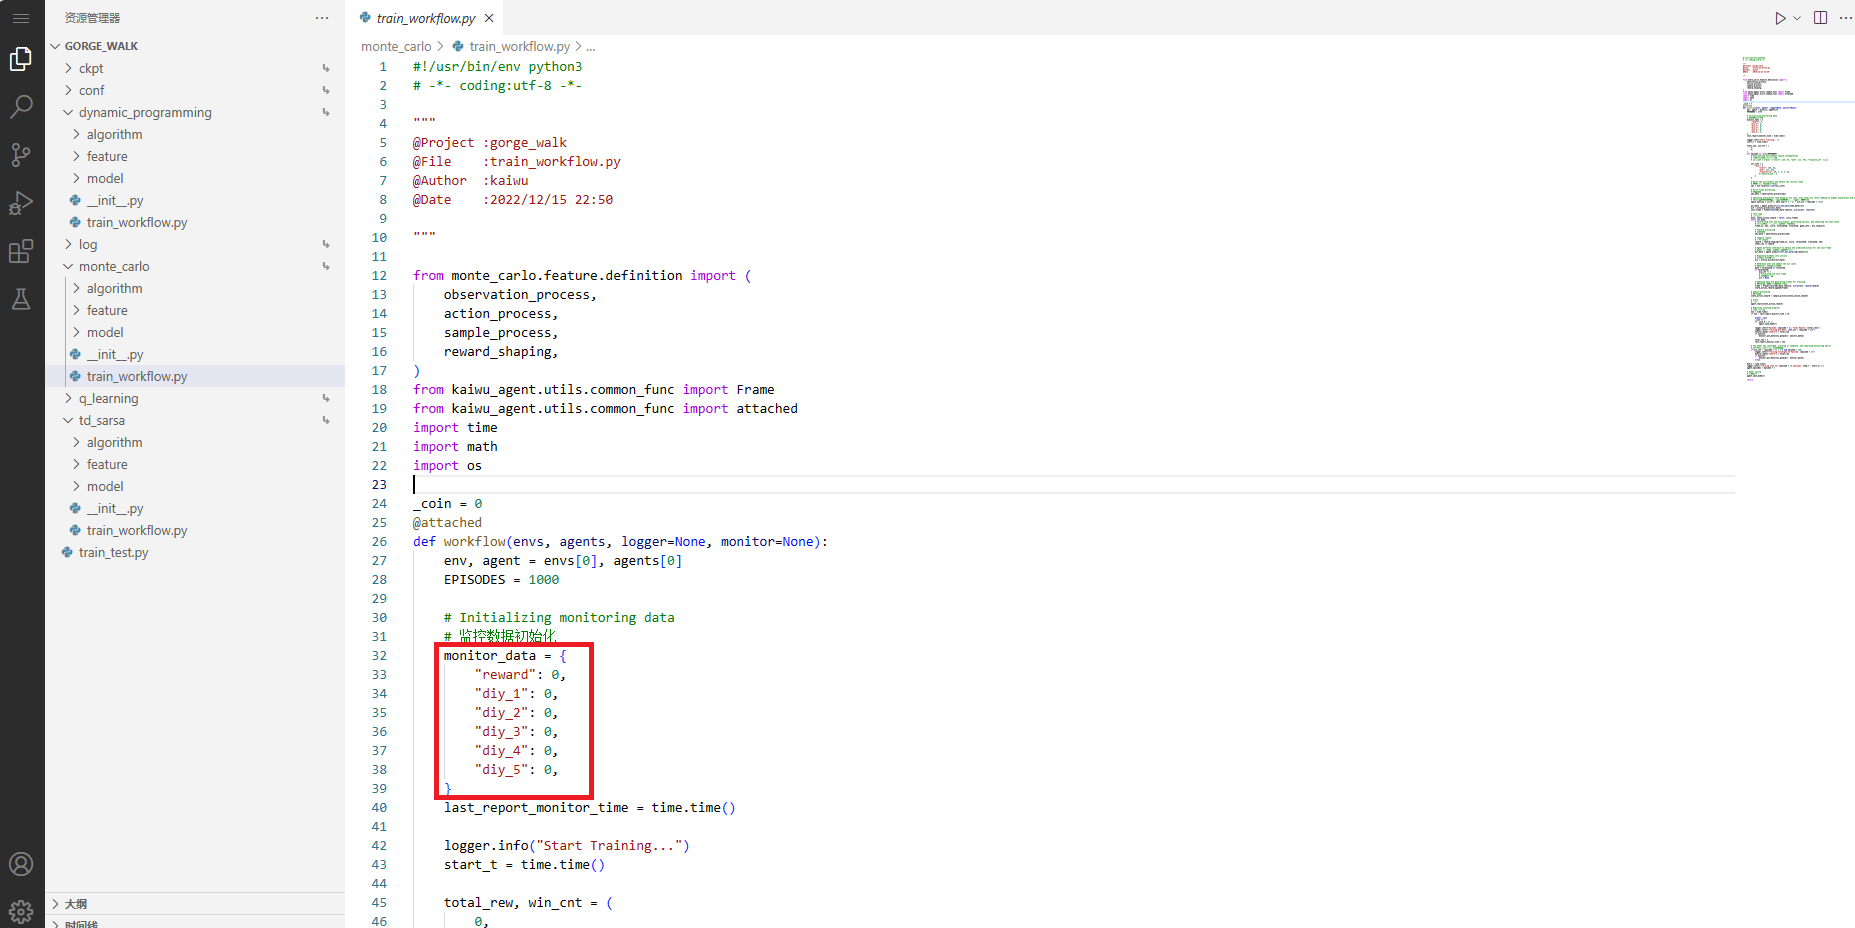
\includegraphics[width=1\linewidth]{pic/diy.png}
        \caption{\zihao{-5} 自定义指标}
        \label{diy}
    \end{figure}

\end{enumerate}

